\documentclass[11pt]{article}
\usepackage{amsmath,amstext,amsfonts,amssymb,amsthm,epsfig,epstopdf,url,array}
\usepackage[margin=1in]{geometry}
\usepackage{xcolor}
\usepackage{graphicx}
\usepackage{times}

\theoremstyle{plain}
\newtheorem{thm}{Theorem}[section]
\newtheorem{lem}[thm]{Lemma}
\newtheorem{prop}[thm]{Proposition}
\newtheorem{cor}[thm]{Corollary}
\newtheorem{defn}[thm]{Definition}
\newtheorem{claim}[thm]{Claim}

\theoremstyle{definition}
\newtheorem{con}{Conjecture}[section]
\newtheorem{exa}{Example}[section]
\newtheorem*{sol}{Solution}
\newtheorem{cdef}{Definition}[section]


\theoremstyle{remark}
\newtheorem{rem}{\textbf{Remark}}
\newtheorem*{note}{\color{blue}\textbf{Note}}
\usepackage{qtree}


\usepackage{hyperref}

\usepackage[nameinlink,noabbrev,capitalize]{cleveref} 
\crefalias{subequation}{equation}
\crefalias{thm}{theorem}


% to make cleveref print ``Lemma'' for lemma
\let\oldlemma\lem
\renewcommand{\lem}{%
  \crefalias{thm}{lem}% Theorem counter now looks like Lemma
  \oldlemma}
\Crefname{lem}{Lemma}{Lemmas}

% to make cleveref print ``Definition for definition
\let\olddefn\defn
\renewcommand{\defn}{%
  \crefalias{thm}{defn}% Theorem counter now looks like Definition
  \olddefn}
\Crefname{defn}{Definition}{Definitions}

% to make cleveref print ``Remark for remark
\let\oldrem\rem
\renewcommand{\rem}{%
  \crefalias{thm}{rem}% Theorem counter now looks like Remark
  \oldrem}
\Crefname{rem}{Remark}{Remarks}

% to make cleveref print ``Corollary for corollary
\let\oldcor\cor
\renewcommand{\cor}{%
  \crefalias{thm}{cor}% Theorem counter now looks like Corollary
  \oldcor}
\Crefname{cor}{Corollary}{Corollaries}

% to make cleveref print ``Claim for claim
\let\oldclaim\claim
\renewcommand{\claim}{%
  \crefalias{thm}{claim}% Theorem counter now looks like Claim
  \oldclaim}
\Crefname{claim}{Claim}{Claims}

% to make cleveref print ``Proposition for prop
\let\oldprop\prop
\renewcommand{\prop}{%
  \crefalias{thm}{prop}% Theorem counter now looks like Prop
  \oldprop}
\Crefname{prop}{Proposition}{Propositions}

% to make cleveref print ``Conjecture for conj
\let\oldcon\con
\renewcommand{\con}{%
  \crefalias{thm}{con}% Theorem counter now looks like Con
  \oldcon}
\Crefname{con}{Conjecture}{Conjectures}

\bibliographystyle{plain}

\begin{document}
\begin{center}
\textbf{Minimum Homotopy Area}
\end{center}



\section*{Abstract}
Systems of quadratic equations appear in several applications from analysis of stochastic processes, machine learning to physical infrastructure systems like the power grid. In recent years, several algorithms have been proposed for the solution of quadratic systems, along with analyses of conditions under which they work. However, in many applications, parameters appearing in the quadratic system of equations are not known perfectly. In these cases, it is of interest to study robust solvability of quadratic systems, that is, whether the quadratic system of equations has a solution (within a certain set) for all realizations within a certain error bound of a given nominal value of the parameters. This problem is NP-hard in general, but we identify special cases that are tractable. Furthermore, we develop a general technique to produce inner and outer bounds on the maximum error bound for which one can guarantee robust solvability (the radius of robust solvability).
The techniques we use combine ideas from constraint programming, convex optimization and topological degree theory. We evaluate our approach numerically on several quadratic systems constructed from the AC power flow equations that describe the steady state of the power grid. The results show that our approach can produce tight lower and upper bounds on the radius of robust solvability.


\section{Introduction}
This paper studies quadratic systems of equations with parameters. More concretely, we study a system of $n$ quadratic equations $F(x)=u$ where $F: \mathbb{R}^n \mapsto \mathbb{R}^n, x,u \in \mathbb{R}^n$ and $F$ is quadratic in $x$. We are interested in situations where the parameters $u$ are uncertain and we are still interested in guaranteeing that there is a solution to $F(x) = u$ for $x$ within limits on $x$ and $u$. Questions of this type arise in a variety of applications from analysis of stochastic processes to infrastructure networks like the power grid and the as grid. For example, in binary markov trees, the parameter $u$ represents the initial probabilities of the Markov chain.

\section{Problem formulation}

\begin{itemize}
\item[] $\mathbb{R}$: Set of real numbers, $\mathbb{R}^n$: $n$-dimensional Euclidean space 
\item[] $\mathbb{S}^n$: Set of $n \times n$ symmetric matrices 
\item[] $\mathbb{R}^{n \times m}$: Set of $n \times m$ real matrices
\item[] $x \in \mathbb{R}^n$): $x$ is a real vector variable
\item[] $M \geq 0$ (for $M \in \mathbb{R}^{n \times n}$): $M$ is a matrix with all entries non-negative  
\item[] $A \in \mathbb{R}^{n\times n}$: $A$ is a potentially sparse condition matrix
\item[] $b \in \mathbb{R}^n$: $b$ is a non-zero vector with all components non-negative
\end{itemize}

We study systems of quadratic equations of the form
\begin{align}
& Q(x)+Lx=u\label{eq:Quad}
\end{align}
where $Q: \mathbb{R}^n \mapsto \mathbb{R}^n$ is a vector-valued quadratic function, that is, there exist symmetric matrices $\mathcal{M}^1,\ldots,\mathcal{M}^{n} \in \mathbb{S}^n$ such that
\[[Q(x)]_i = x^t \mathcal{M}_{i} x \quad \forall i \in [n]\]
and $L \in \mathbb{R}^{n\times n}$ is an $n \times n$ matrix and $u \in \mathbb{R}^n$ is a vector. We are interested in solutions to this system of equations such that
\begin{align}
(Ax)_i\leq b_i \quad \forall i \in [n]\label{eq:xLimits}
\end{align}
However, the parameter $u$ is uncertain and only known upto certain error bounds
\begin{align}
u^{\min}_i=u_i^\star-e_i \leq u_i \leq =u_i^\star+e_i=u^{\max}_i \quad \forall i \in [n] \label{eq:uLimits}
\end{align}
where $u^\star$ is a forecast for $u$ and $e$ denotes the error bounds associated with the forecast. For example, in the case of quadratic equations appearing in infrastructure networks like the power grid, $u_i$ represents uncertain power generation or consumption (for example uncertain weather-dependent power sources like solar or wind power). In the case of stochastic processes, $u^\star$ represents an initial state distribution.

\begin{cdef}[Robust solvability problem]
\label{RobustDef}
Determine whether for all values of $u$ satisfying \eqref{eq:uLimits}, the system of equations \eqref{eq:Quad} has a solution for $x$ satisfying the constraints \eqref{eq:xLimits}. If this is true, the system \eqref{eq:Quad},\eqref{eq:xLimits},\eqref{eq:uLimits} is said to be \emph{robust feasible}. The largest $r$ s.t. $e_i\geq r \ \forall i \ s.t. \ e_i>0$ in \eqref{eq:uLimits} s.t. the system \eqref{eq:Quad},\eqref{eq:xLimits},\eqref{eq:uLimits} is robust feasible is said to be the \emph{robustness margin}.
\end{cdef}

\section{Main technical results}
We now describe the main technical results of this paper. In the first subsection we describe the setting under which the problem can be solved using the results which follow. Our results take advantage of the well studied area of topological degree theory. For an introduction to topological degree theory see {\color{blue}{NEED REFS}}. Suffice it then to say that should $\Omega\in\mathbb{R}^{n}$ be open and bounded, $F:\Omega\rightarrow \mathbb{R}$ continuous, and $F(x)\neq y \quad \forall x\in\partial\Omega$ for some $y\in\mathbb{R}^n$, then $d\left(\Omega,F,y\right)\in\mathbb{Z}$ is defined. 
As in {\color{blue}{Frommer, Hoxha and Lang Thm1}} we utilize the following two results which we form into the following theorem.
\begin{thm} \ \\
\label{thm:Deg}
\begin{itemize}
\item[(i)] If $H : [0,1]\times\bar{\Omega}\rightarrow\mathbb{R}^n$ is continuous such that $H(t,x)\neq y \quad \forall t\in[0,1], \quad x\in\partial\Omega$ then $d\left(\Omega,H(t,\cdot),y\right)$ does not depend on $t$.
\item[(ii)] If $d(\Omega,F,y)\neq 0$, then there exists $x\in\Omega$ s.t. $F(x)=y$.
\end{itemize}

\end{thm}

Our problem necessitates $\Omega=\{x| Ax< b\}$, $F(x)=Q(x)+L(x)$, and a homotopy $H : [0,1]\times\bar{\Omega}\rightarrow\mathbb{R}^n$ defined as 
\begin{align}
H(t,x) = F(x)-t\cdot u \label{eq:Homo}
\end{align}
Observe that by construction $F(\vec{0})=\vec{0}$ and thus $d(\Omega,F(x),\vec{0})\neq 0$. If we wish to guarantee a solution to $F(x)=u$ for some $u\in[u_{min},u_{max}]$ then this is equivalent by (ii) of \cref{thm:Deg} to showing $d(\Omega,H(1,x),\vec{0})\neq 0$. However, by (i) of \cref{thm:Deg}, if it can be shown that $H(t,x)\neq 0, \  \forall t\in[0,1], \  x\in\partial\Omega$, then $d\left(\Omega,H(t,x),0\right)$ does not depend on $t$ and we have that $d\left(\Omega,H(t,x),\vec{0}\right)=d\left(\Omega,H(0,x),\vec{0}\right)=d(\Omega,F(x),\vec{0})\neq 0$. Therefore by \cref{thm:Deg}, it follows that the robust solvability problem can be determined by validating or invalidating the following statement.
\begin{align}
\not\exists x\in\partial\Omega, \ s.t. \ F(x)-u=\vec{0}	 \ \ for \ any \ \ u\in[u_{min},u_{max}]. \label{eq:RSForm}
\end{align}

We now provide results which help derive methods for determining inner and outer approximations on the robustness margin.\\

\begin{lem} \ \\
\label{lem:BdOpt}
Let $X\subset\mathbb{R}^n$ be closed and $\bold{f}:\mathbb{R}^n\rightarrow\mathbb{R}^n$ be continuous. If $\bold{f}$ has no singularities and $$\min\limits_{||\bold{\lambda}||=1}\max\limits_{x\in X}\ \bold{\lambda}^T\bold{f}(x)$$
obtains its optimal at $\bold{\hat{x}}$,$\bold{\lambda}_{\bold{\hat{x}}}$ then $\bold{f}(\bold{\hat{x}})\in \partial \bold{f}(X)$. 

\begin{proof} \ \\
(By contradiction) Assume $\bold{f}(\bold{\hat{x}})\in \bold{f}(X)\setminus\partial \bold{f}(X)$. Let $\theta$ the angle between $\bold{\lambda}_{\bold{\hat{x}}}$ and $\bold{\hat{x}}$. Thus $\min\limits_{||\bold{\lambda}||=1}\max\limits_{x\in X}\ \bold{\lambda}^T\bold{f}(x)=\bold{\lambda}_{\bold{\hat{x}}}^T|\bold{f}(\bold{\hat{x}})|=|\bold{f}(\bold{\hat{x}})|\cos(\theta)$. Since $X\in\mathbb{R}^n$ is closed it is thus compact which implies $\bold{f}(X)$ is also compact. Thus $\exists r>0$ s.t. (ball of radius $r$ centered at $\bold{f}(\bold{\hat{x}})$) $B_r(\bold{f}(\bold{\hat{x}}))\in \bold{f}(X)\setminus\partial \bold{f}(X)$. Let $y$ be the antipodal point on $\partial B_r(\bold{f}(\bold{\hat{x}}))$ to the point of intersection between the line segment connecting the origin to $\bold{f}(\bold{\hat{x}})$ and $B_r(\bold{f}(\bold{\hat{x}}))$. It follows then that $|y|>|\bold{f}(\bold{\hat{x}})|$ and $\theta$ is the angle between $\bold{\lambda}_x$ and $y$.   Let $\bold{x^*}\in X$ s.t. $\bold{f}(\bold{x^*})=y$, such a $\bold{x^*}$ exists as $\bold{f}(X)$ is compact. Therefore $\bold{\lambda}_{\bold{\hat{x}}}^T|\bold{f}(\bold{x^*})|=|\bold{f}(\bold{x^*})|\cos(\theta)>|\bold{f}(\bold{\hat{x}})|\cos(\theta)=\bold{\lambda}_{\bold{\hat{x}}}^T|\bold{f}(\bold{\hat{x}})|$ which is a contradiction. 
The lemma now follows.
\end{proof}
\end{lem}

\begin{thm} \ \\
\label{thm:MainIneq}
Let $X\subset\mathbb{R}^n$ be closed and $\bold{f}:\mathbb{R}^n\rightarrow\mathbb{R}^n$ be continuous s.t. $\bold{f}(X)$ contains the origin. If $\bold{f}$ has no singularities then $$\min\limits_{||\bold{\lambda}||=1}\max\limits_{x\in X}\ \bold{\lambda}^T\bold{f}(x)\geq \min\limits_{x\in \partial X}\max\limits_{||\bold{\lambda}||=1}\ \bold{\lambda}^T\bold{f}(x)$$
\begin{proof} \ \\
If the origin lies on the boundary of $\bold{f}(X)$ then clearly $$\min\limits_{||\bold{\lambda}||=1}\max\limits_{x\in X}\ \bold{\lambda}^T\bold{f}(x)\geq 0 = \min\limits_{x\in \partial X}\max\limits_{||\bold{\lambda}||=1}\ \bold{\lambda}^T\bold{f}(x)$$
Thus assume the origin lies in the interior of $\bold{f}(X)$.
Let $\bold{\hat{x}}$ be the point and $\bold{\lambda}_{\bold{\hat{x}}}$ the unit vector at which $$\min\limits_{||\bold{\lambda}||=1}\max\limits_{x\in X}\ \bold{\lambda}^T\bold{f}(x)$$
obtains its optimal. \\

Case 1: If the angle, $\theta$, between $\bold{\hat{x}}$ and $\bold{\lambda}_{\bold{\hat{x}}}$ is 0 then $\max\limits_{||\bold{\lambda}||=1}\bold{\lambda}^T\bold{f}(\bold{\hat{x}})=\bold{\lambda}_{\bold{\hat{x}}}^T\bold{f}(\bold{\hat{x}})$. Furthermore by \cref{lem:BdOpt} $\bold{f}(\bold{\hat{x}})\in \partial \bold{f}(X)$ and thus $\bold{\hat{x}}\in \partial X$ since $\bold{f}$ has no singularities by hypothesis. It follows now that $$\min\limits_{x\in \partial X}\max\limits_{||\bold{\lambda}||=1}\ \bold{\lambda}^T\bold{f}(x)\leq \bold{\lambda}_{\bold{\hat{x}}}^T\bold{f}(\bold{\hat{x}})=\min\limits_{||\bold{\lambda}||=1}\max\limits_{x\in X}\ \bold{\lambda}^T\bold{f}(x)$$

Case 2: Assume $\theta \neq 0$. Let $\bold{x^*}$ be a point on the boundary of $X$ s.t. the angle between $\bold{\lambda}_{\bold{\hat{x}}}$ and $\bold{f}(\bold{x^*})$ is 0. Such a point must exist as $\bold{f}(X)$ is compact and by hypothesis $\bold{f}(X)$ contains the origin, has no singularities ($\bold{f}$ maps $\partial X$ to $\partial \bold{f}(X)$) and by assumption the origin lies in the interior of $\bold{f}(X)$. It follows then that $$\min\limits_{x\in \partial X}\max\limits_{||\bold{\lambda}||=1}\ \bold{\lambda}^T\bold{f}(x)\leq \max\limits_{||\bold{\lambda}||=1}\bold{\lambda}^T \bold{f}(\bold{x^*}) =\bold{\lambda}_{\bold{\hat{x}}}^T\bold{f}(\bold{x^*})\leq \max\limits_{x\in X}\bold{\lambda}_{\bold{\hat{x}}}^T\bold{f}(x)=\min\limits_{||\bold{\lambda}||=1}\max\limits_{x\in X}\ \bold{\lambda}^T\bold{f}(x)$$

The theorem now follows.

\end{proof}
\end{thm}
\ \\

\subsection{Inner Bound Formulations}

\begin{thm}
Let $\Omega=\{x| Ax< b\}$, $\Omega_{u}=\{u| u^{\min}_i\leq u_i \leq u^{\max}_i \ \forall i \}$, and $F(x)=Q(x)+L(x)$ as described in \eqref{eq:Quad}, \eqref{eq:xLimits} and \eqref{eq:uLimits}. Let
$$z = \min\limits_{x\in \partial \Omega, u\in \Omega_{u} }\max\limits_{||\bold{\lambda}||=1}\ \bold{\lambda}^T\left(F(x)-u\right).$$
If $r>0$ s.t. $r\leq e_i \ \forall i s.t. e_i>0$ where $e$ denotes the error bounds associated with $ u^{\min}_i$ and $ u^{\max}_i$, and if $z>0$ then the system is robust feasible and has a robustness margin of at least r.

\begin{proof} \ \\
If \eqref{eq:RSForm} is invalidated then $\exists \hat{x}\in\partial\Omega$ s.t. $F(\hat{x})=\hat{u}$ for some $\hat{u}\in\Omega_{u}$ and thus $$z = \min\limits_{x\in \partial \Omega}\max\limits_{||\bold{\lambda}||=1}\ \bold{\lambda}^T\left(\bold{F}(x)-u\right)\leq \max\limits_{||\bold{\lambda}||=1, x=\hat{x}}\ \bold{\lambda}^T\left(\bold{F}(x)-\hat{u}\right)=0.$$ 
Hence if $z>0$, \eqref{eq:RSForm} is validated, and the system is robust feasible. It follows then by definition that the system has a robustness margin of at least r.
\end{proof}
\end{thm}


{\color{blue} Need a transition between these theorems. Perhaps $\min\limits_{x\in\partial\Omega_i, u\in \Omega_u} ||F(x)-u||\leq \min\limits_{x\in \partial \Omega, u\in \Omega_{u} }\max\limits_{||\bold{\lambda}||=1}\ \bold{\lambda}^T\left(F(x)-u\right)$ and is easier to calculate.}

\begin{thm} \label{thm:RobFeas}
Let $\partial\Omega_i=\{x| Ax_i = b_i, Ax\leq b\}$, $\Omega_{u}=\{u| u^{\min}_i\leq u_i \leq u^{\max}_i \ \forall i \}$, and $F(x)=Q(x)+L(x)$ as described in \eqref{eq:Quad}, \eqref{eq:xLimits} and \eqref{eq:uLimits}. Define
\begin{align}
\mathrm{z}_i =  \min_{x\in\partial\Omega_i, u\in \Omega_u} ||F(x)-u||. \label{eq:OPTfeas}
\end{align}
If $\mathrm{z}_i>0$ for each $i = 1, \ldots, m$ (where $m$ is the number of rows of $A$), then the system is robust feasible.

\begin{proof} \ \\
If \eqref{eq:RSForm} is invalidated then $\exists \hat{x}\in\partial\Omega$, $\Omega=\{x| Ax< b\}$, s.t. $F(\hat{x})=\hat{u}$ for some $\hat{u}\in \Omega_u$. Since $\hat{x}\in\partial\Omega$ this implies that $\exists i$ s.t. $A\hat{x}_i=b_i$ and thus $0\leq \mathrm{Z}_i \leq ||F(\hat{x})-\hat{u}||=0$. Thus if $\mathrm{Z}_i>0$ for each $i = 1, \ldots, m$ \eqref{eq:RSForm} is validated, and the system is robust feasible as desired.
\end{proof}
\end{thm}

%Note that under these circumstances $\min\limits_{||\bold{\lambda}||=1}\max\limits_{x\in \bar{\Omega}}\ \bold{\lambda}^T\left(\bold{F}(x)-\hat{u}\right)> 0$ is possible, especially if $F(\bar{\Omega})$ is highly non-convex. However, should $\exists u^{\prime}$ s.t. $\min\limits_{||\bold{\lambda}||=1}\max\limits_{x\in \bar{\Omega}}\ \bold{\lambda}^T\left(\bold{F}(x)-u^{\prime}\right)=0$ then by \ref{MainInEqLem} we know that there $\exists \hat{x}\in\partial\Omega$ s.t. $F(\hat{x})=u^{\prime}$. Hence the following formulation of an outer bound approximation on $u_{min}$ and $u_{max}$:


The optimization problems \cref{thm:RobFeas} are nonlinear and nonconvex.
Hence it may be difficult to solve them in general.
However, since $F(x)$ is quadratic in $x$, they are quadratically constrained quadratic programs (QCQPs), and we can use well known \emph{semidefinite programming relaxations for QCQPs} %\cite{d2003relaxations} 
to obtain lower bounds on the optimal values.
Since $Q$ is quadratic, it can also be written as a linear function of $xx^T$.
More concretely, we can write
$$Q(x)_i=x^TM_ix=Trace(M_ixx^T)$$
where each $M_i$ is as defined in \eqref{eq:Quad}. 
Since, $Ax\leq b$ this implies that $(b-Ax)(b-Ax)^T\geq 0\Rightarrow bb^T-Axb^T-b(Ax)^T+A(xx^T)A^T\geq 0$. 
If we allow a symmetric positive semidefinite matrix $X$ to take the place of $xx^T$ we can construct the following relaxation of the model presented in \cref{thm:RobFeas}:
 
\begin{subequations}\label{eq:OPTfeasrelax}
\begin{align}
\hat{\mathrm{z}}_{i} = &\min_x b_i-Ax_i  \\
 \text{subject to: } \ &Tr\left(M\mathcal{X}\right)+q^tx \geq u_{min} \\
 & Tr\left(M\mathcal{X}\right)+q^tx \leq u_{max} \\
 	&Ax\leq b \\
 	&bb^T-Axb^T-b(Ax)^T+A\mathcal{X}A^T\geq O \\
 	&\mathcal{X} \text{ is symmtric, positive semidefinite}
\end{align}
\end{subequations}
where $O$ denotes the $2n \times 2n$ matrix of zeros. This is a convex optimization problem (a semidefinite program, in fact) and can be solved efficiently. Since this is a relaxation of the model in \cref{thm:RobFeas}, if $\hat{\mathrm{z}}_i>0$ for each $i$, the condition in \cref{thm:RobFeas} (i.e. $z_i>0 \ \forall i$) is satisfied. We can further relax the model in \eqref{eq:OPTfeasrelax} by dropping the condition that $X$ be positive semidefinite, which transforms the model from a semidefinite program to a linear program. We now present three formulations for this program that we provide test results for in the next section.

\begin{subequations}\label{eq:OPTfeasrelaxLP1}
\begin{align}
 \text{LP Feasibility Model}& \ z_i  \\
 \text{subject to: } \ &Ax_i= b_i \\
 &Tr\left(M\mathcal{X}\right)+q^tx \geq u_{min} \\
 & Tr\left(M\mathcal{X}\right)+q^tx \leq u_{max} \\
 	&Ax\leq b \\
 	&bb^T-Axb^T-b(Ax)^T+A\mathcal{X}A^T\geq O \\
 	&\mathcal{X} \text{ is symmtric}
\end{align}
\end{subequations}

\begin{subequations}\label{eq:OPTfeasrelaxLP2}
\begin{align}
 \text{MIP Model}& \ \max z  \\
 \text{subject to: } \ &Tr\left(M\mathcal{X}\right)+q^tx \geq u_{min} \\
 & Tr\left(M\mathcal{X}\right)+q^tx \leq u_{max} \\
 	&Ax\leq b \\
 	&bb^T-Axb^T-b(Ax)^T+A\mathcal{X}A^T\geq O \\
 	&\mathcal{X} \text{ is symmtric} \\
 	& z\leq Ax_i-b_i+R(1-d_i) \ \forall i \ \text{ for some large enough $R$} \\
 	& \sum\limits_i d_i=1 \\
 	& d_i\in\{0,1\}
\end{align}
\end{subequations}
 
\begin{subequations}\label{eq:OPTfeasrelaxLP3}
\begin{align}
\text{LP Bound Tightening Model}& \ \mathrm{z}_{i} = \max_x Ax_i  \\
 \text{subject to: } \ &Tr\left(M\mathcal{X}\right)+q^tx \geq u_{min} \\
 & Tr\left(M\mathcal{X}\right)+q^tx \leq u_{max} \\
 	&Ax\leq b \\
 	&bb^T-Axb^T-b(Ax)^T+A\mathcal{X}A^T\geq O \\
 	&\mathcal{X} \text{ is symmtric}
\end{align}
\end{subequations}

The MIP Model and LP Feasibility model are extremely similar and should theoretically give the same results. However, as we will show in our results the LP Feasibility model will out perform the MIP Model in terms of speed. Of particular interest is the LP Bound Tightening Model, which can be used in the same manner as the LP Feasibility model except instead of finding a feasible solution at each dimension one simply checks to ensure $Ax_i <b_i$. What distinguishes the LP Bound Tightening model, however, is its ability to be used iteratively by updating the constraints \eqref{eq:OPTfeasrelaxLP3}[d\& e] by replacing $b$ with $z$ (the vector of $z_i$'s found after running the model over all dimensions of $Ax$). Since clearly $b\leq z$ we have that the polytope $\{Ax\leq z\}\subseteq\{Ax\leq b\}$. Thus it follows that any system deemed robust feasible using \eqref{eq:OPTfeasrelaxLP1} or \eqref{eq:OPTfeasrelaxLP2} would certainly be found robust feasible using \eqref{eq:OPTfeasrelaxLP3}, but a system found robust feasible using \eqref{eq:OPTfeasrelaxLP3} may not be found robust feasible using \eqref{eq:OPTfeasrelaxLP1} or \eqref{eq:OPTfeasrelaxLP2}. 


\subsection{Outer Bound Formulations}

As a result of the complexity of $\min\limits_{x\in \partial \Omega, u\in\Omega_u}\max\limits_{||\bold{\lambda}||=1}\ \bold{\lambda}^T\left(F(x)-u\right)$ we derived a sequence of relaxations in order to arrive at a method that was computationally efficient for a non-trivial data set. We can similarly work with $\min\limits_{||\bold{\lambda}||=1}\max\limits_{x\in \bar{\Omega}, u\in\Omega_u}\ \bold{\lambda}^T\left(F(x)-u\right)$ to produce computationally efficient models for outer bound approximations of the robustness margin. \\
\begin{thm}\label{thm:OPTfeasOut} 
Let $\bar{\Omega}=\{x| Ax\leq b\}$, $\Omega_{u}=\{u| u^{\min}_i\leq u_i \leq u^{\max}_i \ \forall i \}$, and $F(x)=Q(x)+L(x)$ as described in \eqref{eq:Quad}, \eqref{eq:xLimits} and \eqref{eq:uLimits}. Let
$$z = \min\limits_{||\bold{\lambda}||=1}\max\limits_{x\in \bar{\Omega}, u\in\Omega_u}\ \bold{\lambda}^T\left(F(x)-u\right).$$
If $r>0$ s.t. $r\leq e_i \ \forall i \ s.t. \ e_i>0$ where $e$ denotes the error bounds associated with $ u^{\min}_i$ and $ u^{\max}_i$, and if $z>0$ then the system is robust feasible and has a robustness margin of at least r.

\begin{proof} \ \\
Observe by \cref{lem:BdOpt} that if $\min\limits_{||\bold{\lambda}||=1}\max\limits_{x\in \Omega, u\in\Omega_u}\ \bold{\lambda}^T\left(F(x)-u\right)=0$, then \eqref{eq:RSForm} is validated. Observe that if \eqref{eq:RSForm} is invalidated then $\exists \hat{x}\in\partial\Omega$ s.t. $F(\hat{x})=\hat{u}$ for some $\hat{u}\in\Omega_{u}$ and thus certainly $$\min\limits_{||\bold{\lambda}||=1}\max\limits_{x\in X, u\in\Omega_u}\ \bold{\lambda}^T\left(F(x)-u\right) \geq \min\limits_{||\bold{\lambda}||=1}\ \bold{\lambda}^T\left(F(\hat{x})-\hat{u}\right)=0.$$ The theorem now follows.
\end{proof}
\end{thm}

We can relax the model in \cref{thm:OPTfeasOut} utilizing the same techniques as before, replacing $xx^T$ with a positive semidefinite matrix $X$, with the option of dropping the condition that $X$ be positive semidefinite, which transforms the model from a semidefinite program to a linear or mixed integer program depending on how one deals with the condition $||\bold{\lambda}||=1$. 

\begin{subequations}\label{eq:OPTfeasOutRelaxa}
\begin{align}
\text{Outer Bound Model A}& \ \min\limits_{||\bold{\lambda}||=1}\max\limits_{x}  \\
 \text{subject to: } \ & Ax\leq b \\
 	&bb^T-Axb^T-b(Ax)^T+A\mathcal{X}A^T\geq O \\
 	&\mathcal{X} \text{ is symmtric}
\end{align}
\end{subequations}

We can construct the dual of the inner maximal objective of \eqref{eq:OPTfeasOutRelaxa} to produce:

\begin{subequations}\label{eq:OPTfeasOutRelaxb}
\begin{align}
\text{Outer Bound Model B}& \ \min\limits_{||\bold{\lambda}||=1,y}B^Ty  \\
 \text{subject to: } \ & H^Ty=u(\lambda) \\
 & y\leq 0
\end{align}
where \eqref{eq:OPTfeasOutRelaxa}$[b \& c]$ can be written as $Hx\geq B$ and the objective of \eqref{eq:OPTfeasOutRelaxa} as $u(\lambda)^Tx$.
\end{subequations}


\section{Numerical studies}
We now present computational studies which support the efficiency of the models we have presented. For all the numerical results presented we apply our models to find upper and lower bounds for the robustness margins with respect to the optimal power flow equations derived using datasets obtained from the MatPower package found in the MATLAB software. We will specifically show results for tests conducted on cases 5, 9, 14, 30 and 57. In every case the power flow equations were converted into the format defined by \eqref{eq:Quad}, \eqref{eq:xLimits}, and \eqref{eq:uLimits}. To simulate real life scenarios we allowed the first 5 dimensions of $u$ to represent renewable energy, and the others representing no variation. We then slowly increased the variation of the first 5 dimensions of $u$, while utilizing models \eqref{eq:OPTfeasOutRelaxb} for the outer bound, and \eqref{eq:OPTfeasrelaxLP1}, \eqref{eq:OPTfeasrelaxLP2} and \eqref{eq:OPTfeasrelaxLP3} for the inner bound verification to verify robust feasibility. The results are presented in table {\color{blue}Need table ref} where each row of the table represents results conducted with $Ax\leq b = B*ones$ for $B\in\{0.001, 0.005,0.01\}$ and $ones$ representing the vector of all ones of appropriate dimension. $A$ in this cases is a matrix s.t. $Ax\leq b$ controls the flow between nodes in the power grid (i.e. each row of $Ax\leq b$ has the form $x_i-x_j\leq b_k$. All computations were performed on a laptop running the 64bit Windows 10 operating system containing an Intel i-7 processor, 16 GB of Ram and 4 cores.\\

\begin{table}[h]
\begin{center}
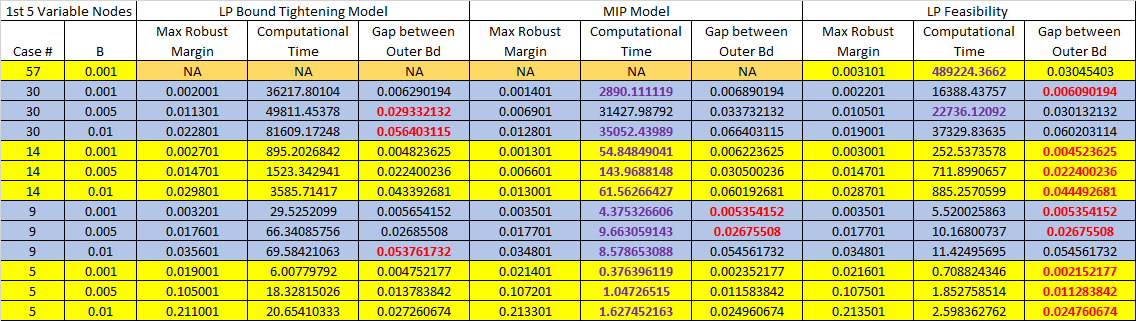
\includegraphics[scale=0.5]{Figures/InnerBoundTable}
\caption{Robustness Margins for inner bound models } 
\vspace{0.2in}
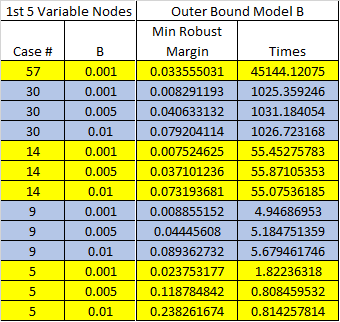
\includegraphics[scale=0.5]{Figures/OuterBoundTable}
\caption{Robustness Margins for outer bound models}
\end{center}
\end{table} 

Graphically we can look at this data on a case by case basis to highlight the effect of allowing more fluctuation between the nodes (i.e. as $B$ increases). \\

\begin{figure}[h]
\begin{center}
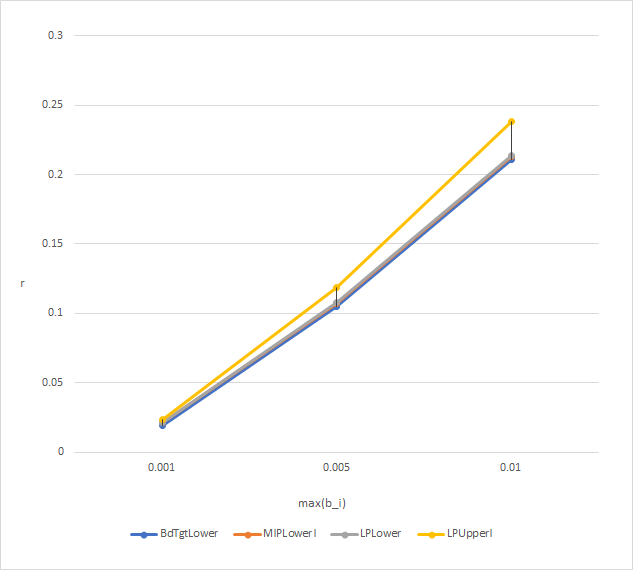
\includegraphics[scale=0.4]{Figures/Case5}
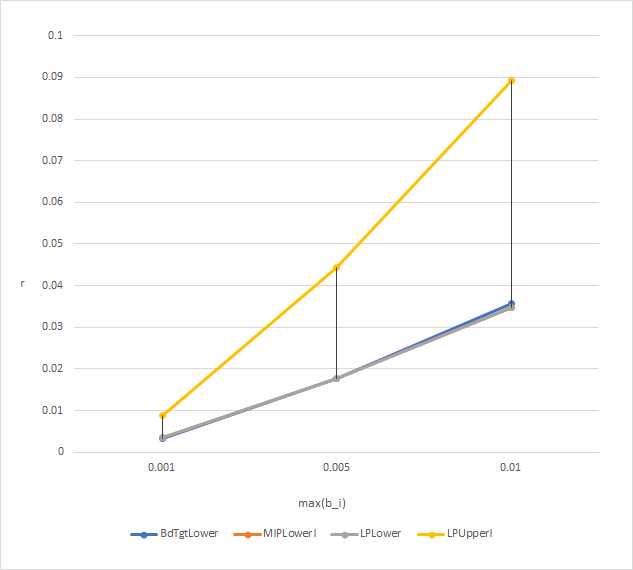
\includegraphics[scale=0.4]{Figures/Case9} \\
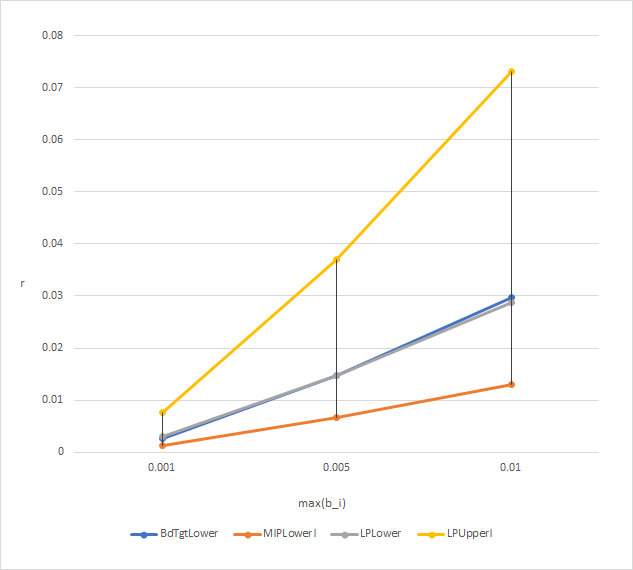
\includegraphics[scale=0.4]{Figures/Case14}
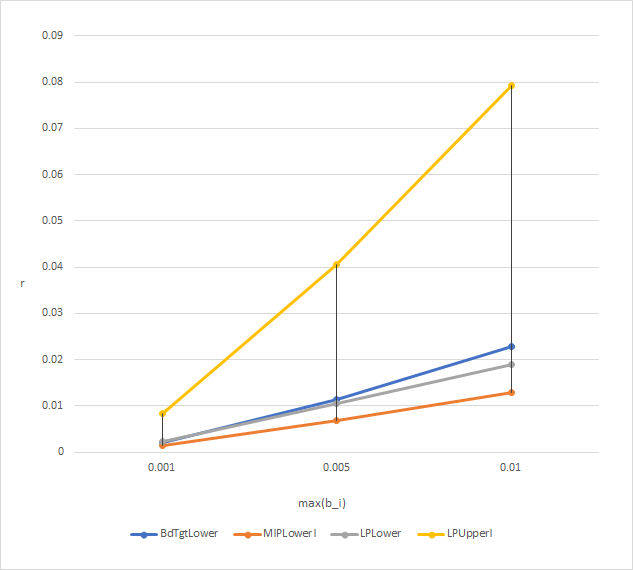
\includegraphics[scale=0.4]{Figures/Case30}
\caption{Case 5 (Top Left), Case 9 (Top Right), Case 14 (Bottom Left), Case 30 (Bottom Right)}
\end{center}
\end{figure} 

\newpage

As evident from the table we have that the bound tightening model produces a better approximation of the inner bound on the robustness margin as the complexity of the data set increases. Certainly one would expect the bound tightening model to out perform the other inner bound models for all cases, but the choice of model parameters has a big effect on the efficiency of the model. For instance, setting a low tolerance for a minimal sufficient change in the dimensions of $b$ will cause in most cases an extremely long running time. Thus in the lower complexity cases it should be expected that the other models will out perform the bound tightening model as these manually set model parameters will have more of an impact on performance. \\
Of special interest is the difference in performance of the MIP and Feasibility inner bound models as the complexity of the data increases. In particular it was surprising that the Feasibility model was the only inner bound model capable of efficiently computing the robustness margin for case 57. 


\section{Conclusion}

We have successfully proposed novel and efficient techniques for determining robust solvability of quadratic systems in this paper. It is worth mentioning that the same machinery can be used to determine robustness margins of solutions to static systems by taking $A$ to be the identity, $e_i=0 \ \forall i$ and simply adjusting $b$ accordingly. The models presented here are in some sense just the tip of the iceberg. More efficient models can certainly be derived using the theory contained here. We present these models only as examples of how efficient algorithms could be constructed utilizing the theoretical results present here. \\



\end{document}